%-------------------------------------------------------------------------
%-------------------------------------------------------------------------
%-------------------------------------------------------------------------
\section{Methodology}
\iffalse
\TODO{Some parts of the methodology are very complex. While this is not a problem in itself, there is sometimes no motivation in the paper for the introduction of these complexities. For example, equations 2.4, 2.5, 2.6 and 2.7 represent the affinities between mesh nodes, but only a small amount of justification is given for these formulae ­­­ e.g. what is the benefit of using a Geman­McClure robust function?}
\TODO{The benefit of segmenting the images rather than the mesh is not immediately clear. The images are segmented using an existing technique for short­baseline video, ignoring the PTAM output and the meshed reconstruction of the scene. The individual image segmentations are then projected into the mesh using the known camera poses. These different segmentations are then combined. The benefits of doing this, rather than alternatives such as segmenting the mesh directly should be made clear through explanation and/or qualitative and quantitative evaluation. The proposed algorithm seems to suggest that two identical meshes reconstructed from different input video sequences could be given very different final segmentations. Is that true, and why is that desirable?}
\fi
%-------------------------------------------------------------------------
\subsection{Scene Model}\label{sec:sceneModel}
\iffalse
\tc{A lot of this math is unnecessary noise in your description. When you
introduce notation, if you only use it once or twice, it's probably better
to just leave it out and describe things in words.}
\fi
The input to our system is a grayscale video $\{I_t\}_{t = 0}^T$, with each image
$I_t$ mapping from a domain $D\subset\real^2$ to $\real_+$. 
The desired output is a constant partitioning of a
higher-dimensional ``scene'' that the video observes, from which we can also derive a piecewise-constant,
integer-valued function 
%\mbox{$c:D\times [0, T] \rightarrow {\mathbb Z}; (x,t) \mapsto 
{$c_t(x)$} that associates to each pixel $x\in D$ a label. The scene is
represented
by a (multiply-connected) collection of surfaces $S \subset \real^3$ supporting a reflectance
function (albedo) $\rho : S \rightarrow \real_+$. 
Under the Lambert-Ambient model, the image and the scene are related by
\begin{equation}
\begin{cases} I_t(x) = \rho(p) + n_t(x), \ p \in S \\ x = \pi(g_t p) + v_t(x)
\end{cases}
\end{equation}
where $g_t \equiv (R(t), T(t)) \in SE(3)$ is the pose of the camera relative to
the reference frame of $S$, and $\pi:\real^3 \rightarrow D$ is a canonical
central (perspective) projection. The residual $n_t(x)$ accounts for unmodeled
photometric phenomena such as changes in illumination (assumed negligible in the
short time-span during which the video is captured), deviations from Lambertian
reflection, sensor noise etc. The residual $v_t(x)$ accounts for violations of
the geometric assumptions (rigid motion, static scene). Estimates $\hat g_t, \hat S$ are
obtained as described in Sec. \ref{sec:densemonoc}.

We consider that objects in the scene compose a nested covering of sets $\S = \{S_i\}_{i = 1}^K$, 
where $S_i \cap S_j \in \{\emptyset, S_i, S_j\}$ for all $i$ and $j$, and $\bigcup_{i=1}^K S_i=S$. 
%Some of the objects may correspond to a connected component of $S$, but others may split or share multiple components. 
Any segmentation of the scene is a selection $\P = \{S_{\P,i}\}_{i=1}^{K_\P}$
of disjoint sets in $\S$ such that $\bigcup_{i=1}^{K_p}S_{\P,i} = S$. For a partitioning
$\P$ to be meaningful, typically some homogeneity property must hold on each $S_{\P,i}$, 
be that geometric, photometric, semantic, topological, or some combination. 
%The value of introducing the scene $S$ to our model of video segmentation is that it allows us to {\em
%avoid inferring complex and discontinuous deformations of $D_{\P,i}(t) := \pi(g_t S_{\P,i}) \cap D$, and
%instead produce estimates of the partitions $\P\subs\S$, and hence $\S$, directly.} 
%\TODO{Use this notation for image segmentation section}
 %(here, out-of-frame or occluded points map to $\emptyset$).
%\footnote{Note that the projection function $\pi:\real^3_+\to D$ hides the computation of {\em visibility}, as only the
%segments of the scene that are visible contribute to the segmentation of the video. This depends on
%both the shape of the scene $S$ and the motion of the viewer $g_t$. As such, it is invertible on $\D$--that is,
%for each $x\in D$, we can find unique $p\in\RR^3_+$ such that $\pi(g_t p) = x$.}

One can perform a sequence of still-frame (or short-baseline video) segmentations 
%For the task of scene-segmentation-from-video, we wish to derive an object-segmentation $\P$ from a sequence of 
$c_t:D\to\mathbb{Z}^+$ using a subset of these properties
which can then be leveraged into a segmentation of the scene.
A reasonable such segmentation is one that does not oversegment the scene relative to $c_t$
(distinguish points that have the same label $c_t$ for all or almost all $t$),
or undersegment (fail to distinguish points that tend to have different labels), more than necessary.
As these $c_t$ will be temporally inconsistent, they can be regularized by integration on the scene 
using geometric homogeneity.
We consider a particular set of segmentations $c_t$ to induce a selection $\P$ from $\S$.
The use of occlusion-based image segmentation (Sec. \ref{sec:signatures})
to induce a segmentation respecting topological homogeneity as seen by the viewer
is a key contribution of our approach.

\iffalse
Ideally, for any two points $x_1,x_2\in D$, there exist $i$ and $j$ such that
\begin{align}
&c_{t}(x_1) = c_{t}(x_2) = j \notag \\ 
&\quad\iff g_t^{-1}(\pi^{-1}x_1), g_t^{-1}(\pi^{-1}x_1) \in S_{\P,i}. \label{eq:derived_partition}
\end{align}
(the correspondence between scene-components $i$ and image-components $j$ may be arbitrary).  If only the forward 
implication holds, we say that $c_t$ is an oversegmentation.  If only the reverse, $c_t$ is an undersegmentation.
%Given a perfect segmentation $c$, the best we can hope for is
%\begin{align}
%&c_{\P,t}(x_1) = c_{\P,t}(x_2) = j \notag \\ 
%&\quad\iff g_t^{-1}(\pi^{-1}x_1), g_t^{-1}(\pi^{-1}x_1) \in S_{\P,i}.
%\end{align}
Often, however, there exist no partitions of $\P$ that satisfy (\ref{eq:derived_partition}) for all $t$.
Thus it is desirable to define a ``best'' partition of the scene, which tries to minimize both under- and oversegmentation.  
\fi

\iffalse
We propose the following:
\def\Q{\mathcal{Q}}
\begin{align}
\P &= \underset{\text{partitions $\Q$ of $S$}}{\argmin} 
\sum_{p,q\in\S} 
\begin{cases}\!\!
\begin{smallmatrix}
1 & p\sim q\text{ in $\Q$}\\
-1 & p\not\sim q\text{ in $\Q$}
\end{smallmatrix}
\end{cases}\notag\\
&\qquad\qquad\biggl(
\bigl|\bigl\{t: c_t(\pi(g_t p))\neq c_t(\pi(g_t q))\bigr\}\bigr|
\end{equation}
\fi

%Thus, we can re-formulate the task as {\em given} $\{I_t\}_{t =
%1}^T$ {\em and} $\hat g_t, \hat S$, {\em partition} the scene into components
%$\{S_i\}$ and the corresponding $\rho_i$, that are {\em geometrically and/or
%photometrically} distinct from their neighborhood. 
%\TODO{Topologically from the viewer? Can we use this motivate the adaptive geodesic?}


\subsection{Curvature Augmented Geometry and Geometric Affinity}
Here we discuss the construction of a 3D mesh representation of the scene, and 
of an augmented geometry for curvature-based affinity computations.
%-------------------------------------------------------------------------
\subsubsection{Dense Monocular Reconstruction}\label{sec:densemonoc}
A estimate of the scene $\hat S$ is reconstructed in an on-line fashion as the camera browses the
scene. We use the real-time camera tracking system PTAM \cite{Klein2007}, a fast dense
stereo module, and a globally optimal depth map fusion algorithm. The latter component takes as
input depth maps and camera poses obtained from the former components, and computes a dense surface using an implicit volumetric representation via a
truncated signed distance function (TSDF), similar to \cite{Zach2007,Zach2008,Graber2011}. Dense depth maps are computed using multiview plane-sweeping \cite{Collins1996} on a set of images and their camera poses obtained from the tracking module. The main advantage of this
approach is that it allows for arbitrary scene topology. It is also closely related to the Kinect
Fusion \cite{Newcombe2011a}, although we do not employ a depth sensor but work solely based on image
data. 
Example surface normal and depth maps extracted from our dense reconstruction are shown in figure
\ref{fig:normal_depth}.

%%%%The planesweep algorithm
%%%%computes the best match in a cost volume, where we used a $3\times 3$ zero-mean sum of absolute
%%%%differences (SAD) for computing the cost function. For memory and performance
%%%%reasons, we do not store the cost-volume but instead compute the minimum on-the-fly as we sweep
%%%%through the planes. Using a parallel GPU implementation this results in a very fast algorithm where
%%%%we can use a large number of frames for computing the depth map.
%%%%
%%%%The goal of depth map fusion is to find the TSDF $u$ that best agrees with an
%%%%arbitrary number of measurements (i.e. depth maps).
%%%%We start by converting depth maps to
%%%%TSDF-fields $f_i:R\mapsto [-1, 1]$, where $R \subseteq \Omega$ is the part of the volume
%%%%that is seen by the depth map.
%%%%The conversion involves projecting voxels into the
%%%%depth map according to $x=\pi(gp)$, whereby
%%%%$x\in D$ are the projected pixel coordinates, $\pi : \mathbb{R}^3
%%%%\rightarrow \mathbb{R}^2$ is the projection onto the image plane given by the camera calibration
%%%%parameters, $g \in SE(3)$ is the camera pose of the depth map reference frame and $p\in\Omega$
%%%%is a world point in the volume of interest.
%%%%The value of the TSDF is then
%%%%found by comparing the depth of the world point $p$ from the depth map camera position
%%%%to the measurement in the depth map at the pixel
%%%%position $x$.
%%%%
%%%%Next, we use the following convex approach for fusion of the distance fields
%%%%\cite{Graber2011}
%%%%\begin{equation}
%%%%\label{eq:5}
%%%%\min_u \int_\Omega |\nabla u| + \lambda \sum_{b=1}^{B} \int_\Omega h(p,b) |u-d(b)|~ \mathrm{d}p
%%%%\end{equation}
%%%%We use a TV regularizer with $\nabla$ denoting the distributional derivative, which minimizes the
%%%%total surface area of the final 3D model. The dataterm employs a robust $\ell_1$-norm and
%%%%penalizes deviations of the surface $u$ from the TSDF-fields $f_i$.
%%%%
%%%%Note that since \eqref{eq:5} is convex, we are able to compute the optimum
%%%%independent from any
%%%%initialization. In particular, we can continuously add new data as it becomes
%%%%available (i.e. as the
%%%%camera explores the scene and depth maps are generated), and the algorithm adapts
%%%%the solution
%%%%accordingly. This can be seen as kind of an online learning of the scene
%%%%geometry. For optimization of
%%%%\eqref{eq:5}, we again employ the primal-dual algorithm \cite{Chambolle2011}.


For the purposes of computing affinities between points on $\hat S$, we construct discretized mesh derived from the
regular voxelization of the reconstructed scene. Affinities between regions of the scene can be
computed as functions of the nodes of this mesh. Each node $q$ aggregates the spatial information (mean location, mean normal, Sec. \ref{sec:curvGeod}) and image-based topological cues (Sec. \ref{sec:signatures}) of the surfaces passing through the associated voxel.

\begin{figure}
\begin{center}
  \centerline
      {
        \hbox
            {%\\
              \begin{tabular}{cc}
		{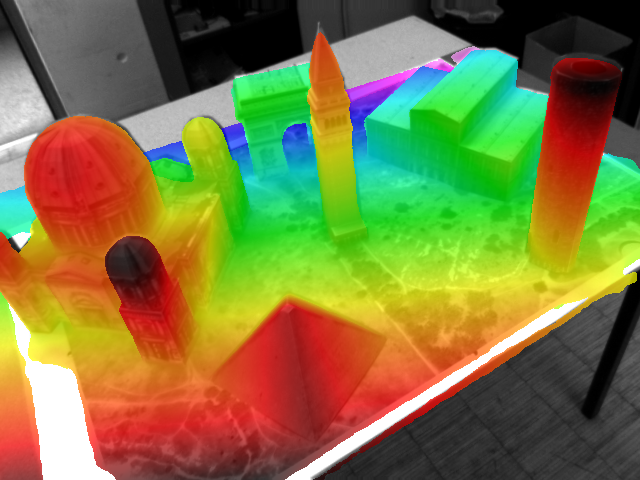
\includegraphics[width=0.48\textwidth]{figs/cos/depth.png}}
		{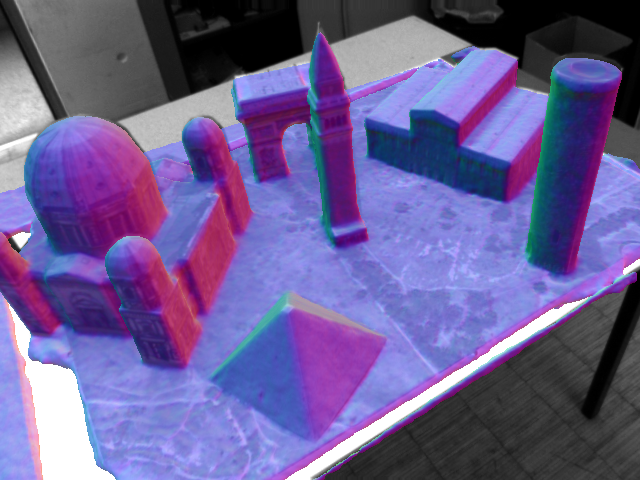
\includegraphics[width=0.48\textwidth]{figs/cos/normal.png}}
		\\
		{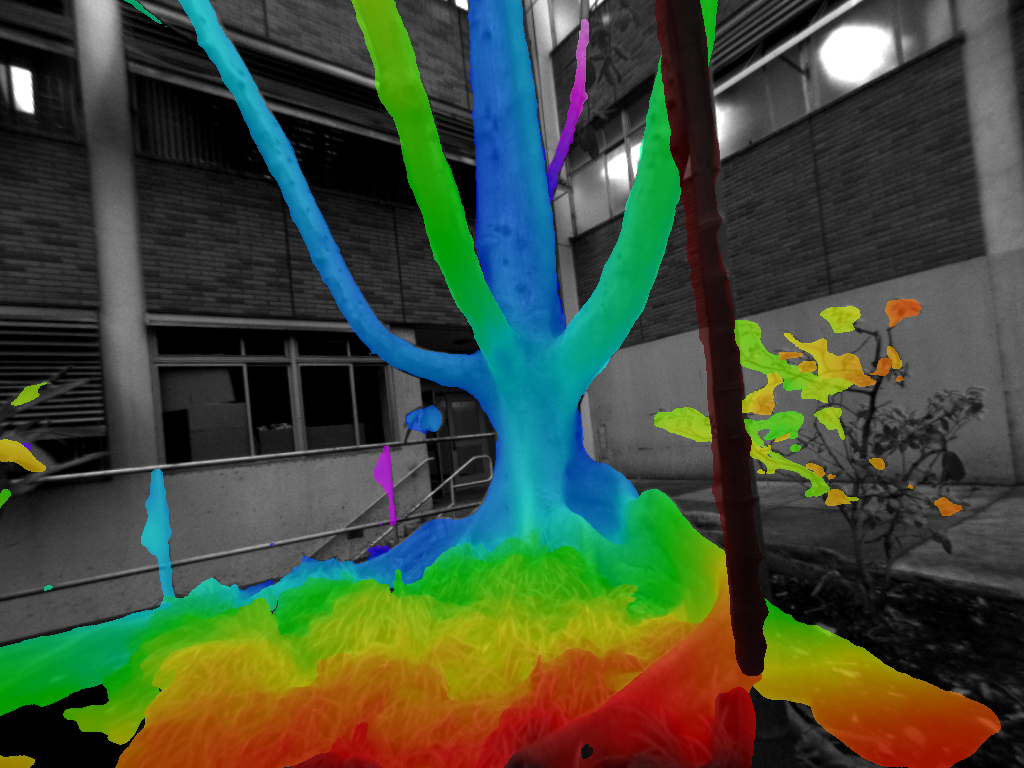
\includegraphics[width=0.48\textwidth]{figs/park4/depth.png}}
		{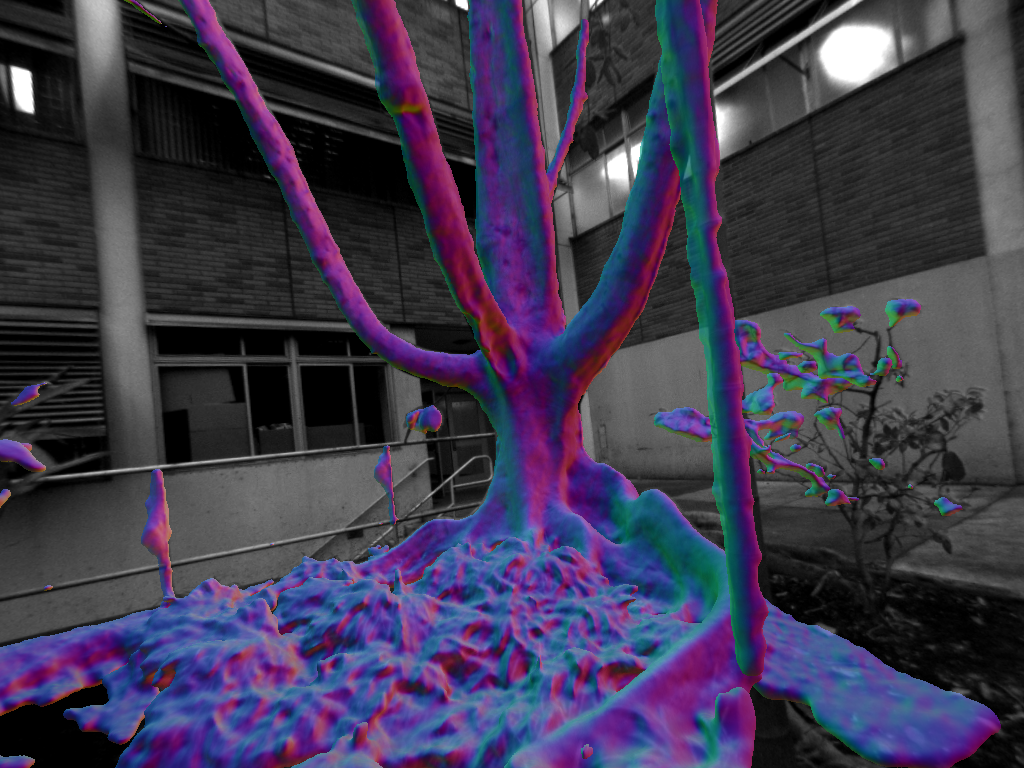
\includegraphics[width=0.48\textwidth]{figs/park4/normal.png}}
		\\
		{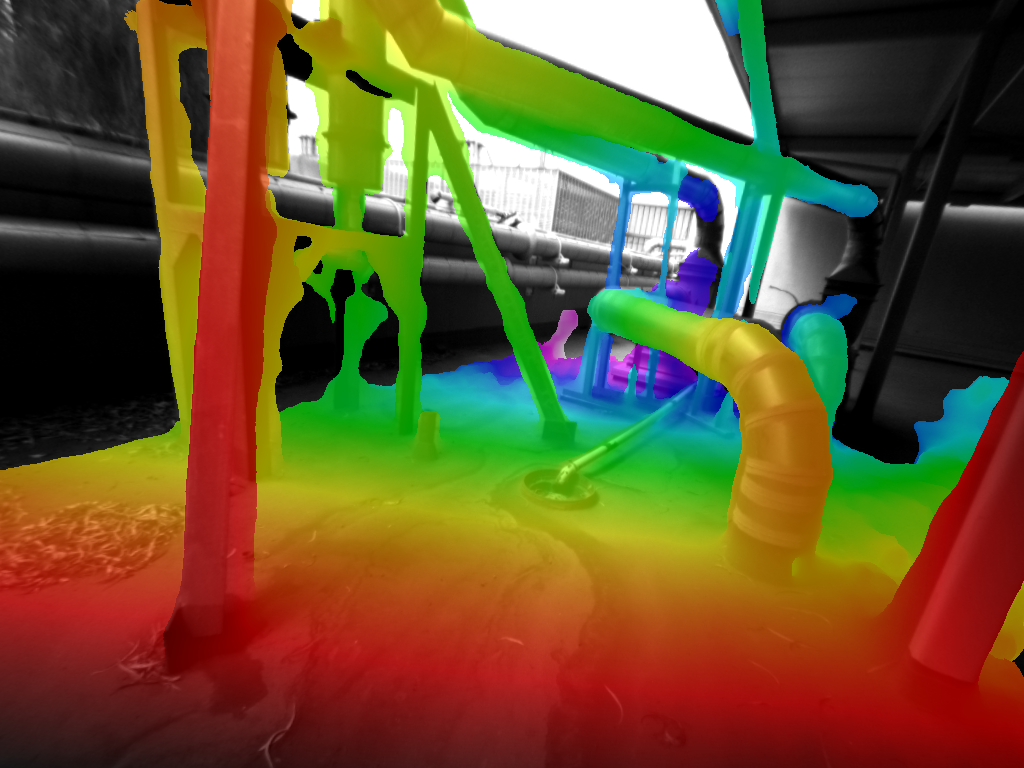
\includegraphics[width=0.48\textwidth]{figs/pipes2/depth.png}}
		{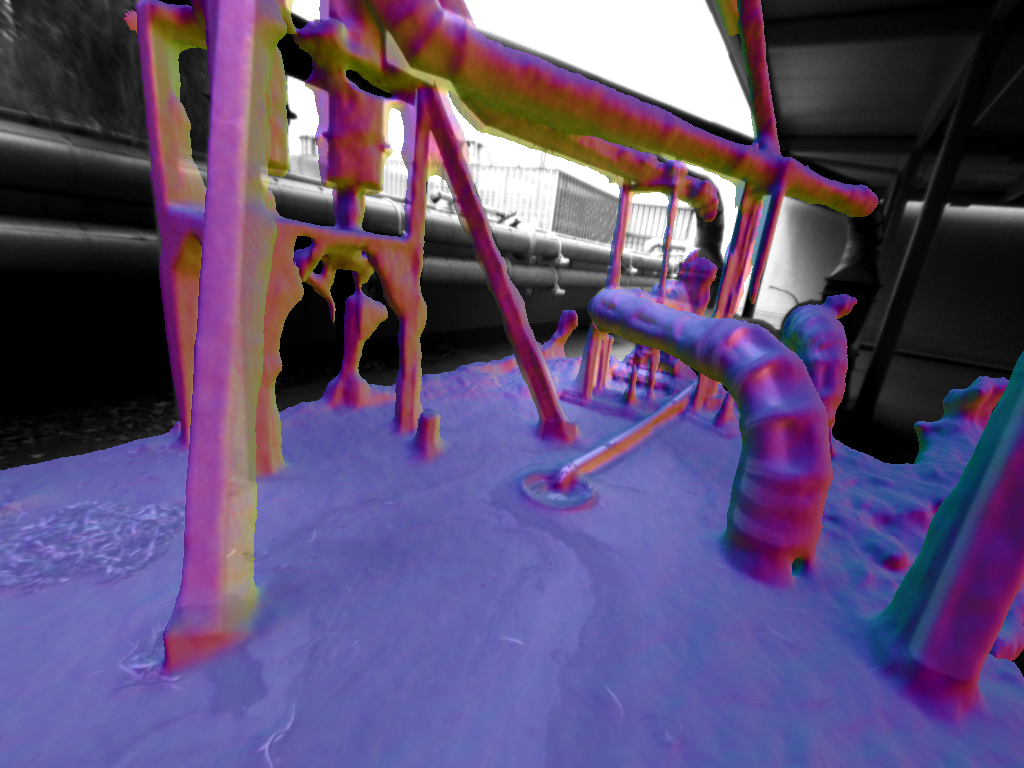
\includegraphics[width=0.48\textwidth]{figs/pipes2/normal.png}}
		\\
		{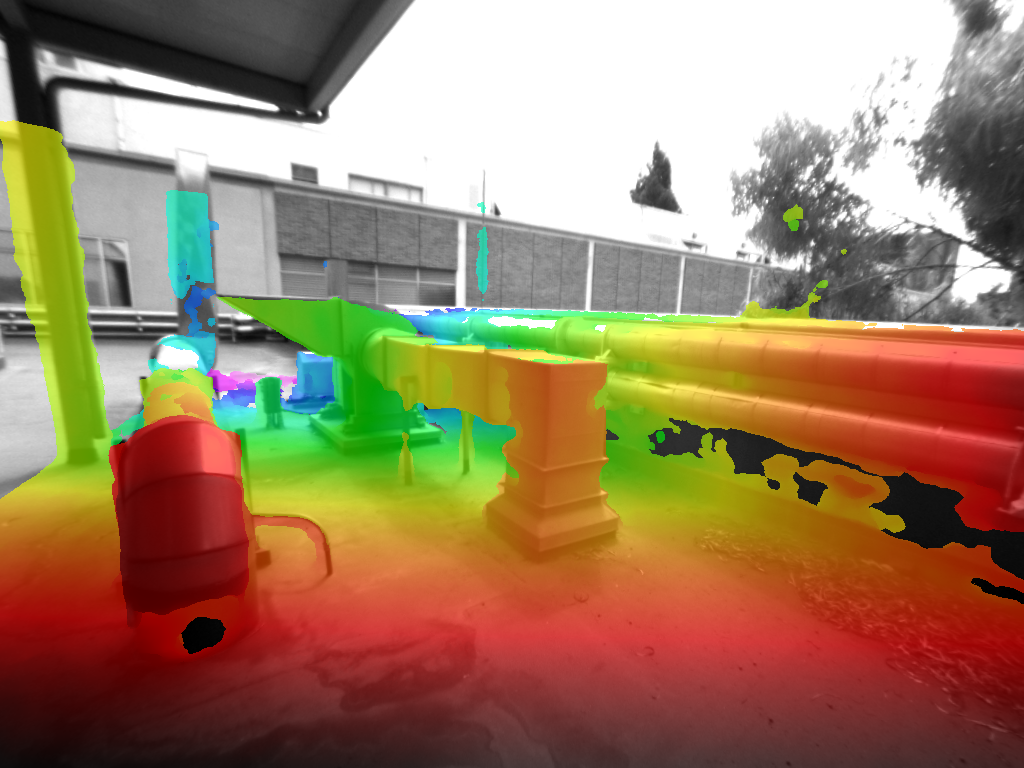
\includegraphics[width=0.48\textwidth]{figs/pipes3/depth.png}}
		{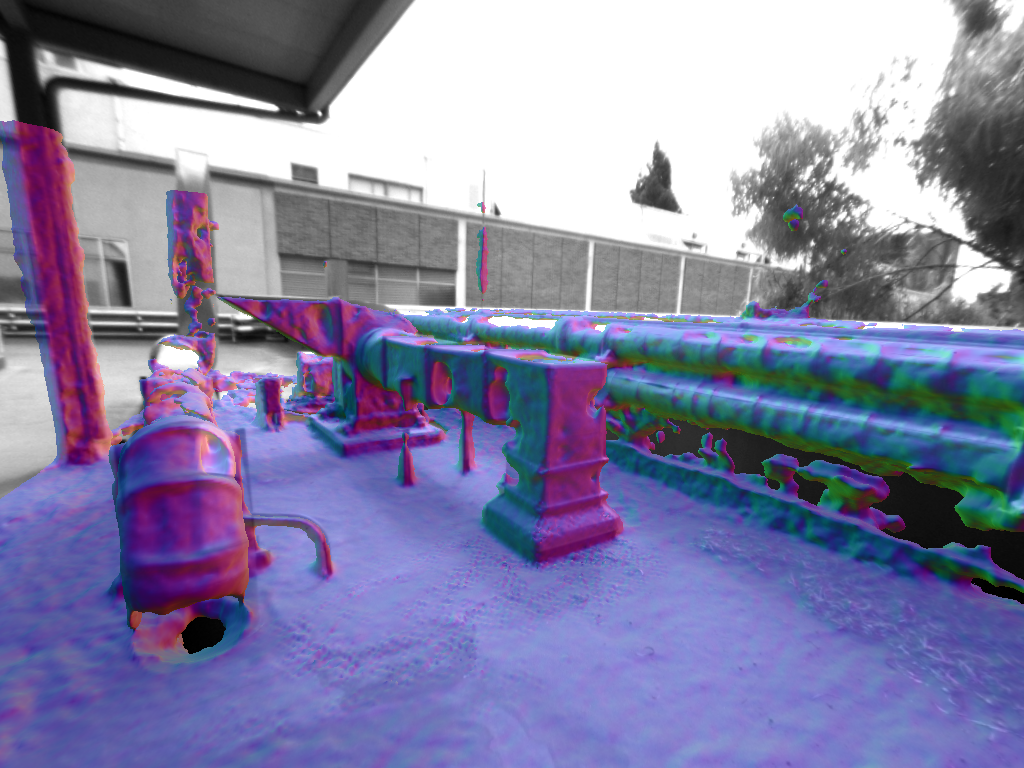
\includegraphics[width=0.48\textwidth]{figs/pipes3/normal.png}}
              \end{tabular}
            }
      }
\end{center}
{}
   \caption{\small Dense reconstructions of indoor and outdoor scenes from monocular video:
   depth (left column) and normal (right column) maps.
   From top: \emph{City of Sights}, \emph{Tree}, \emph{Industrial1}, \emph{Industrial2}
(described in section \ref{sec:results}).}
\label{fig:normal_depth}
{}
\end{figure}
